\documentclass{article}
\usepackage{arxiv}

\usepackage[utf8]{inputenc}
\usepackage[english, russian]{babel}
\usepackage[T1]{fontenc}
\usepackage{url}
\usepackage{booktabs}
\usepackage{amsfonts}
\usepackage{nicefrac}
\usepackage{microtype}
\usepackage{lipsum}
\usepackage{graphicx}
\usepackage{natbib}
\usepackage{doi}
\usepackage{color}
\usepackage{xcolor}

\newcommand{\TODO}[1]{\textcolor{purple}{ToDo: #1.}}

\title{Binary Neural Networks. Lossless picture quality for binary neural networks in pixel-level tasks.}

\author{Kirill Ovcharenko \\
	Moscow Institute of Physics and Technology\\
	%% examples of more authors
	\And
	Zharikov Ilya \\
	Moscow Institute of Physics and Technology\\
	%% \AND
	%% Coauthor \\
	%% Affiliation \\
	%% Address \\
	%% \texttt{email} \\
	%% \And
	%% Coauthor \\
	%% Affiliation \\
	%% Address \\
	%% \texttt{email} \\
	%% \And
	%% Coauthor \\
	%% Affiliation \\
	%% Address \\
	%% \texttt{email} \\
}
\date{}

\renewcommand{\shorttitle}{\textit{arXiv} Template}

%%% Add PDF metadata to help others organize their library
%%% Once the PDF is generated, you can check the metadata with
%%% $ pdfinfo template.pdf
\hypersetup{
pdftitle={A template for the arxiv style},
pdfsubject={q-bio.NC, q-bio.QM},
pdfauthor={David S.~Hippocampus, Elias D.~Striatum},
pdfkeywords={First keyword, Second keyword, More},
}

\begin{document}
\maketitle

\begin{abstract}
Image Super Resolution [SR] is a crucial class of image processing techniques that enhance quality of visual data. 
Deep Convolutional Neural Networks [DCNN] have recently shown great results in this field. However, application of DCNN on resource-limited devices remains challenging, as they demand significant amounts of memory, energy and computations. Binary neural networks [BNN] provide a promising approach to reduce computational complexity and speed up the inference of a model. To our best knowledge, there are not many papers devoted to applying BNN to SR tasks, as SR models are much more vulnerable to degradation in performance when decreasing the precision of weights, than image classification models. The paper proposes modification of a convolutional block to make it binary without performance decreasing.

\end{abstract}


\keywords{Binary Neural Network \and Single Image Super Resolution \and Binarization \and Model compression}

\section{Introduction}

\TODO{Need to be extended in terms related works further}

Image Super Resolution [SR] aims to restore High Quality [HQ] image from corrupted Low Quality [LQ] counterpart. This task is important because of its various applications in medical imaging and surveillance instruments. In spite of the research in this field being active, it made some progress not a long ago, as some challenges were encountered. Main obstacle is desired output in SR tasks being much more diverse than input, so the model is required to do dense pixel-level prediction, hence is bound to be more complex.  

Recent advances in the field of SR owe their success to Deep Neural Networks [DNN] which show state-of-the-art results in a wide range of computer vision problems, such as image classification, Semantic Segmentation etc. However, the models solving these tasks are usually complicated and demand a lot of space and computational resources, thus hindering their implementation on mobile devices, drones and other machines which are limited in GPU memory.

Lately, different methods of reducing complexity of these models were proposed. While some papers focus on pruning and knowledge distillation, other researches introduce quantization as a way to decrease memory needed.

The most extreme form of quantization is binarization. Binary Neural Networks [BNN] use only $1$ bit to represent each parameter, thus drastically decreasing space demanded to store the model. Moreover, with all parameters of the model set to $\{-1, 1\}$, most of the the calculations can be conducted using XNOR and Bitcount operations. This approach seems promising, as it proposes new ways to design hardware that can help to handle and exploit complex neural networks.

However, it is obvious that BNN sacrifice precision and quality, as they have much less capacity and representational potential than Full-Precision [FP] networks. Previous works in this field propose different methods of maintaining competitive accuracy while achieving better performance. The paper~\cite{ma2019efficient} focuses on residual block binarization, which helps to reduce a significant part of the model's parameters. However, full-precision activations keep computational complexity of the model pretty high. ReactNet~\cite{liu2020reactnet} suggests generalized binarization and activations functions that help to shift distribution, which significantly increases representational capacity of the binary model. The BBCU~\cite{xia2022basic} proposed effective Convolutional Unit that can be used in any architecture that relies on residual connections. It provides much more efficient training and inference, but oversimplifies weight binarization. IR-Net~\cite{qin2020forward} reduces information loss by balancing weights to achieve maximum information entropy in forward propagation. After that, IR2Net~\cite{xue2022ir2net} proposes two essential components of the learning process: Information Restriction and Information Recovery. BNext~\cite{guo2022join} also applies attention mechanism to obtain the key information from the full-precision activations. 
However, last two papers investigate only the impact of these methods on performance of Image Classification models. However, the paper~\cite{zhao2020efficient} presented a new method of attention that exhibits great results in SR task.

This paper adopts some techniques from the researches, mentioned above, and suggests further modifications of convolutional block that help to improve BNN's performance in SR tasks.

We use EDSR~\cite{lim2017enhanced} as a backbone for our modified binary block, as it doesn't require batch normalization block and shows state-of-the-art results. We use BBCU~\cite{xia2022basic} as a baseline for our modification as it showed prominent performance in multiple Image Restoration tasks, particularly in SR. This paper proposes several adjustments for the binary convolutional block.

Firstly, we adopt the idea of using generalized activation and sign functions from \cite{liu2020reactnet}. That helps to achieve better performance while preserving competitive quality. 

Secondly, we keep the idea of updating full-precision weights with respect to binarized weights from ~\cite{ma2019efficient}. We also maintain a learnable scale factor in contrast to ~\cite{xia2022basic}, where the optimal value is used, because the former method was proven to give better results.

Finally, we advance the idea from ~\cite{xue2022ir2net} and ~\cite{guo2022join} to restrict information from the input to increase learning productivity by implementing attention modules into our binary network. We try different ways to compute attention maps, including the method proposed in ~\cite{zhao2020efficient}.

\section{Problem statement}
\label{sec:headings}

\TODO{Need to be slightly reformulated during theory week}

Let $\{(X_i, Y_i)\}_{i=1}^n$ be our image dataset, where $X_i \in \mathbb{R}^{h_i \times w_i \times 3}$ denotes the low resolution image and $Y_i \in \mathbb{R}^{H_i \times W_i \times 3}$ - the high resolution one. Considering $M$ to be the model, SR task targets optimization of 
\begin{equation}
    Q(M) = \frac{1}{n}\sum\limits_{i=1}^nf(M(X_i), Y_i)
\end{equation}
where $f$ represents either $PSNR$ or $SSIM$ metric, defined as:
\begin{equation}
    PSNR(x, y) = 10 \log_{10} \left(\frac{MAX_I^2}{MSE(x, y)}\right)
\end{equation}


Here $MAX_I$ is the maximum valid value for pixel, $MSE$ is mean squared error.

\begin{equation}
    SSIM(x, y) = \frac{(2\mu_x\mu_y + c_1)(2\sigma_{xy} + c_2)}{(\mu_x^2 + \mu_y^2 + c_1)(\sigma_{x}^2 + \sigma_{y}^2 + c_2)}
\end{equation}

$\mu_x$ denotes the mean for $x$, $\mu_y$ - the mean for $y$, $\sigma_x$ is the variance for $x$, $\sigma_y$ is the variance for $y$, $\sigma_{xy}$ is the covariation of $x$ and $y$, $c_1$ and $c_2$ - two constants depending on dynamic pixel range.

Now let $B \in \mathcal{B}$ be our binarized representation of model $M$. $\mathcal{B}$ is space of BNN. Assuming $L$ to be number of layers in $B \in \mathcal{B}$, $W_l \in \{-1, 1\}^{C_{out} \times C_{in} \times K_h \times K_w}$, $l \in \{1 \ , ... \ , L\}$. Here $C_{out}$ is the number of output channels, $C_{in}$ is the number of input channels, $K_h$ is the kernel height, $K_w$ is the kernel weight. 


Thus, the problem of binarization can be expressed in finding $B^{*}$ as
\begin{equation}
    B^{*} = \arg\min\limits_{B \in \mathcal{B}} \left[Q(M) - Q(B)\right]
\end{equation}

\section{Basic Binary Convolutional Block modification}

\subsection{Generalized activation functions}
\subsection{Learnable scale factor}
\subsection{Attention module for binary block}

\section{Computational experiment}
\subsection{Preliminary report}
\begin{figure}[h]
\caption{Validation metric plots for baseline (BBCU)}
\centering
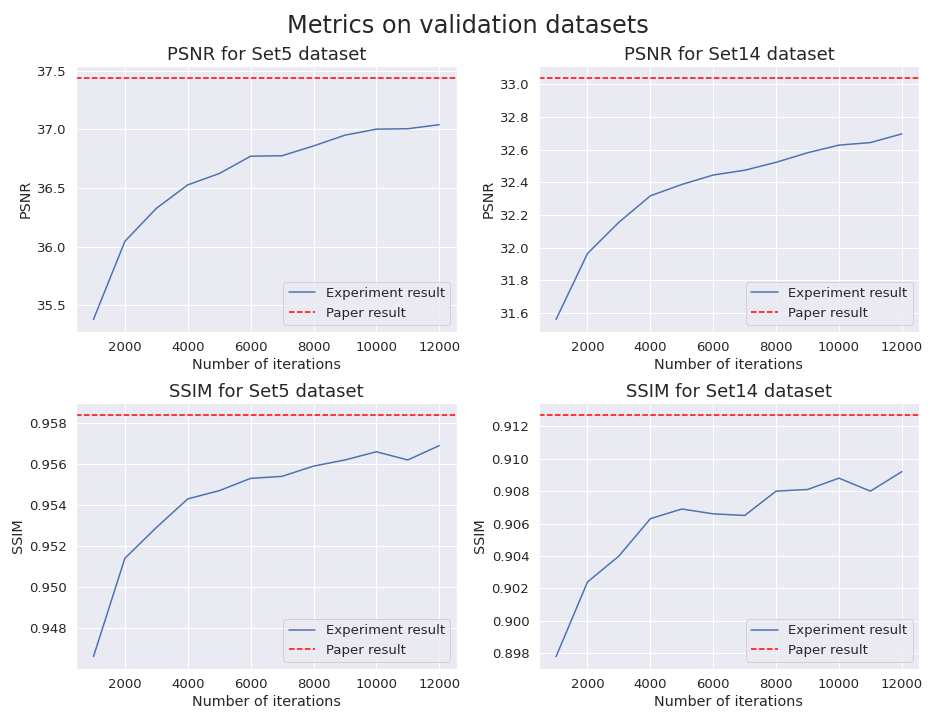
\includegraphics[width=0.8\textwidth]{val_metrics.png}
\end{figure}
We expect our modification to show the same trend of PSNR and SSIM metrics, but the goal of the research is to increase the performance while preserving the amount of computational resources required.


\bibliographystyle{unsrtnat}
\bibliography{references}

\end{document}